\documentclass[../main-sheet.tex]{subfiles}
\usepackage{../style}
\graphicspath{ {../img/} }
\backgroundsetup{contents={}}
\begin{document}
\chapter{Transportation Problem}
The transportation model is a special class of the linear programming problem. It deals with the situation in which a commodity is shipped from \emph{sources} (e.g., factories) to \emph{destinations} (e.g., warehouses). The objective is to determine the amounts shipped from each sources to each destination that minimize the total shipping cost while satisfying both the supply limits and the demand requirements. The model assumes that the shipping cost on a given route is directly proportional to the number of units shipped on that route.\\

Suppose that there are \(m\) sources and \(n\) destinations. Let \(a_i\) be the number of supply units available at source \(i\,(i=1,2,\dots,m)\) and let \(b_j\) be the number of demand units required at destination \(j\, (j=1,2,\dots,n)\). Let \(c_{ij}\) represent the unit transportation cost for transporting the units from source \(i\) to destination \(j\). Then, if \(x_{ij}\) \((x_{ij}>0)\) is the number of units shipped from source \(i\) to destination \(j\), the problem is to determine the Transportation schedule so as to minimize the total transportation cost satisfying the supply and demand conditions.

Mathematically, the problem may be stated as follows:
\begin{mini*}
    {}{Z=\sum_{i=1}^m \sum_{j=1}^n c_{ij}x_{ij}}{}{}
    \addConstraint{x_{i1}+x_{i2}+\dots+x_{in}}{=a_i;\quad i=1,2,\dots,m\quad \Rightarrow \sum_{j=1}^n x_{ij}=a_i}
    \addConstraint{x_{1j}+x_{2j}+\dots+x_{mj}}{=b_i;\quad j=1,2,\dots,n\quad \Rightarrow \sum_{i=1}^m x_{ij}=b_j}
    \addConstraint{x_{ij}}{\geq 0;\quad \text{for all }i\text{ and }j}
\end{mini*}
For a feasible solution to exist, it is necessary that total supply equals total requirement i.e.,
\[
    \sum_{i=1}^m a_i=\sum_{j=1}^n b_j
\]
This restriction causes one of the constraints to be redundant (and hence it can be deleted) so that the problem will have \((m+n-1)\) independent constraints and \((m\times n)\) unknowns.
\begin{note}
    The standard transportation problem has \((m+n)\) constraint, \(mn\) variables. In general, the number of basic variables in a basic feasible solution is given by the number of constraints. Nut in the TP, the number of variables that can take positive values is limited \((m+n-1)\), since
    \[
        \sum_{i=1}^m\sum_{j=1}^n x_{ij}=\sum_{i=1}^m a_i\qquad\text{ and }\qquad\sum_{j=1}^n\sum_{i=1}^m x_{ij}=\sum_{j=1}^n b_j
    \]
    Also, we have that \(\sum_{i=1}^m a_i=\sum_{j=1}^n b_j\) and hence, the transportation model have only \((m+n-1)\) independent constraints.
\end{note}
\section{Starting Basic Feasible Solution}
To solve a standard TP, we shall use the following methods (for starting basic feasible solution):
\begin{enumerate}
    \item North-west corner rule (NCR)
    \item Least-cost rule (LCR)
    \item Vogel's approximation rule/method (VAM)
\end{enumerate}
\begin{prob}
    Consider a transportation problem with 3 warehouses and 4 markets. The warehouse capacities are \(a_1=3,\;a_2=7,\;a_3=5\). The market demands are \(b_1=4,\;b_2=3,\;b_4=4\). The unit cost of shipping is given by the following table:
    \begin{figure}[H]
        \centering
        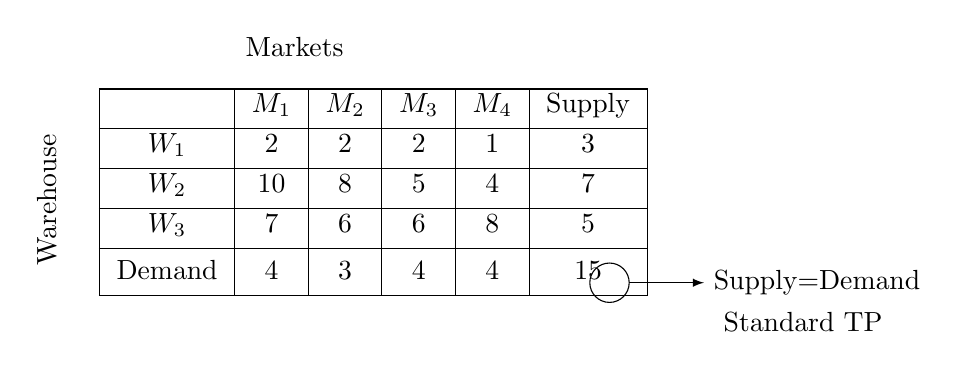
\begin{tikzpicture}
            \node at (0,0) {
                \begin{tabular}[t]{|c|c|c|c|c|c|}
                    \hline 
                       & $M_1$ & $M_2$ & $M_3$ & $M_4$ & Supply  \\[2pt] 
                       \hline
                    $W_1$   & 2    & 2    & 2    & 1    & 3      \\[2pt] \hline
                    $W_2$   & 10   & 8    & 5    & 4    & 7      \\[2pt] \hline
                    $W_3$   & 7    & 6    & 6    & 8    & 5      \\[2pt] \hline
                    \rule{0pt}{11pt}Demand & 4    & 3    & 4    & 4    & 15     \\[2pt] \hline
                \end{tabular}
            };
            \node at (-1,1.85) {Markets};
            \node [rotate=90] at (-4.15,-.1) {Warehouse};
            \draw (3,-1.15) circle (.25);
            \draw[-latex](3.25,-1.15)--(4.2,-1.15)node[right]{Supply=Demand};
            \node at (5.4,-1.65) {$\therefore$ Standard TP};
            \end{tikzpicture}
    \end{figure}
\end{prob}
\begin{soln}
    In this transportation problem,
    \[\sum_{i=1}^3 a_i =\sum_{j=1}^4 b_j=15\]
    So, it is a standard TP.\\
    The transportation table is as follows:
    \begin{table}[H]
        \centering
        \begin{tabular}{|c|cc|cc|cc|cc|c|}
        \hline
         & \multicolumn{2}{c|}{$M_1$} & \multicolumn{2}{c|}{$M_2$} & \multicolumn{2}{c|}{$M_3$} & \multicolumn{2}{c|}{$M_4$} & Supply \\[2pt] \hline
        \multirow{2}{*}{$W_1$} & 3 &  &  &  &  &  &  &  & \multirow{2}{*}{\cancel{3}} \\ \cline{3-3} \cline{5-5} \cline{7-7} \cline{9-9}
         & \multicolumn{1}{c|}{} & 2 & \multicolumn{1}{c|}{} & 2 & \multicolumn{1}{c|}{} & 2 & \multicolumn{1}{c|}{} & 1 &  \\ \hline
        \multirow{2}{*}{$W_2$} & 1 &  & 3 &  & 3 &  &  &  & \multirow{2}{*}{\cancel{7} \cancel{6} \cancel{3}} \\ \cline{3-3} \cline{5-5} \cline{7-7} \cline{9-9}
         & \multicolumn{1}{c|}{} & 10 & \multicolumn{1}{c|}{} & 8 & \multicolumn{1}{c|}{} & 5 & \multicolumn{1}{c|}{} & 4 &  \\ \hline
        \multirow{2}{*}{$W_3$} &  &  &  &  & 1 &  & 4 &  & \multirow{2}{*}{\cancel{5} \cancel{4}} \\ \cline{3-3} \cline{5-5} \cline{7-7} \cline{9-9}
         & \multicolumn{1}{c|}{} & 7 & \multicolumn{1}{c|}{} & 6 & \multicolumn{1}{c|}{} & 6 & \multicolumn{1}{c|}{} & 8 &  \\ \hline
        Demand & \multicolumn{2}{c|}{\cancel{4} \cancel{1}} & \multicolumn{2}{c|}{\cancel{3}} & \multicolumn{2}{c|}{\cancel{4} \cancel{1}} & \multicolumn{2}{c|}{4} &  \\[2pt] \hline
        \end{tabular}
        \end{table}
        Here, we shall refrain from writing the variable names \(x_{ij}\).\\
        A basic feasible solution to this problem will have at most \((3+4-1)=6\) positive variables.
\end{soln}
\subsection{North-west corner Rule}
This rule generates a feasible solution with no more than \((m+n-1)\) basic variables.

Here \(x_{11}\) is selected as the 1st basic variable and is assigned a value as much as possible consistent with the supply and demand restriction.\\
Set \(x_{11}=\min\{3,4\}=3\). We set the variable \(x_{12}=x_{13}=x_{14}=0\). The remaining demand of the market \(M_1\) is 1 unit. The next variable \(x_{21}\) and \(x_{21}=\min\{7,1\}=1\).\\
Similarly, \(x_{22}=\min\{6,3\}=3\)\\
In the same manner, finally we obtain the table-2.
\begin{table}[H]
    \centering
    \begin{tabular}{|c|cc|cc|cc|cc|c|}
    \hline
     & \multicolumn{2}{c|}{$M_1$} & \multicolumn{2}{c|}{$M_2$} & \multicolumn{2}{c|}{$M_3$} & \multicolumn{2}{c|}{$M_4$} & Supply \\[2pt] \hline
    \multirow{2}{*}{$W_1$} & 3 &  &  &  &  &  &  &  & \multirow{2}{*}{3} \\ \cline{3-3} \cline{5-5} \cline{7-7} \cline{9-9}
     & \multicolumn{1}{c|}{} & 2 & \multicolumn{1}{c|}{} & 2 & \multicolumn{1}{c|}{} & 2 & \multicolumn{1}{c|}{} & 1 &  \\ \hline
    \multirow{2}{*}{$W_2$} & 1 &  & 3 &  & 3 &  &  &  & \multirow{2}{*}{7} \\ \cline{3-3} \cline{5-5} \cline{7-7} \cline{9-9}
     & \multicolumn{1}{c|}{} & 10 & \multicolumn{1}{c|}{} & 8 & \multicolumn{1}{c|}{} & 5 & \multicolumn{1}{c|}{} & 4 &  \\ \hline
    \multirow{2}{*}{$W_3$} &  &  &  &  & 1 &  & 4 &  & \multirow{2}{*}{5} \\ \cline{3-3} \cline{5-5} \cline{7-7} \cline{9-9}
     & \multicolumn{1}{c|}{} & 7 & \multicolumn{1}{c|}{} & 6 & \multicolumn{1}{c|}{} & 6 & \multicolumn{1}{c|}{} & 8 &  \\ \hline
    Demand & \multicolumn{2}{c|}{4} & \multicolumn{2}{c|}{3} & \multicolumn{2}{c|}{4} & \multicolumn{2}{c|}{4} &  \\[2pt] \hline
    \end{tabular}
    \caption{tab-2}
\end{table}
Since we have six positive variables in the solution, so for the initial basic feasible solution, the total cost is given by
\[
    Z=3\cdot2+1\cdot10+3\cdot8+3\cdot5+1\cdot6+4\cdot8=93
\]
\subsection{Least Cost Rule (LCR)}
In this rule, the variable with the least shipping cost will be chosen as the basic variable.

According to this rule, in our present problem \(x_{14}\) must be chosen as the 1st basic variable, and \(x_{14}=\min\{3,4\}=3\).
\begin{table}[H]
    \centering
    \begin{tabular}{|c|cc|cc|cc|cc|c|}
    \hline
                           & \multicolumn{2}{c|}{$M_1$} & \multicolumn{2}{c|}{$M_2$} & \multicolumn{2}{c|}{$M_3$} & \multicolumn{2}{c|}{$M_4$} & Supply             \\ \hline
    \multirow{2}{*}{$W_1$} &                       &    &                        &   &                        &   & 3                      &   & \multirow{2}{*}{\cancel{3}} \\ \cline{3-3} \cline{5-5} \cline{7-7} \cline{9-9}
                           & \multicolumn{1}{c|}{} & 2  & \multicolumn{1}{c|}{}  & 2 & \multicolumn{1}{c|}{}  & 2 & \multicolumn{1}{c|}{}  & 1 &                    \\ \hline
    \multirow{2}{*}{$W_2$} & 2                     &    &                        &   & 4                      &   & 1                      &   & \multirow{2}{*}{\cancel{7} \cancel{6} \cancel{2}} \\ \cline{3-3} \cline{5-5} \cline{7-7} \cline{9-9}
                           & \multicolumn{1}{c|}{} & 10 & \multicolumn{1}{c|}{}  & 8 & \multicolumn{1}{c|}{}  & 5 & \multicolumn{1}{c|}{}  & 4 &                    \\ \hline
    \multirow{2}{*}{$W_3$} & 2                     &    & 3                      &   &                        &   &                        &   & \multirow{2}{*}{\cancel{5} \cancel{2}} \\ \cline{3-3} \cline{5-5} \cline{7-7} \cline{9-9}
                           & \multicolumn{1}{c|}{} & 7  & \multicolumn{1}{c|}{}  & 6 & \multicolumn{1}{c|}{}  & 6 & \multicolumn{1}{c|}{}  & 8 &                    \\ \hline
    Demand                 & \multicolumn{2}{c|}{\cancel{4} \cancel{2}}     & \multicolumn{2}{c|}{\cancel{3}}     & \multicolumn{2}{c|}{\cancel{4}}     & \multicolumn{2}{c|}{\cancel{4} \cancel{1}}     &                    \\ \hline
    \end{tabular}
\end{table}
Now, out of the remaining unassigned cells, the variable \(x_{24}\) has the least cost and \(x_{24}=\min\{7,1\}=1\).

In this way, finally, we obtain the following table which gives the initial basic feasible solution.
\begin{table}[H]
    \centering
    \begin{tabular}{|c|cc|cc|cc|cc|c|}
    \hline
                           & \multicolumn{2}{c|}{$M_1$} & \multicolumn{2}{c|}{$M_2$} & \multicolumn{2}{c|}{$M_3$} & \multicolumn{2}{c|}{$M_4$} & Supply             \\ \hline
    \multirow{2}{*}{$W_1$} &                       &    &                        &   &                        &   & 3                      &   & \multirow{2}{*}{3} \\ \cline{3-3} \cline{5-5} \cline{7-7} \cline{9-9}
                           & \multicolumn{1}{c|}{} & 2  & \multicolumn{1}{c|}{}  & 2 & \multicolumn{1}{c|}{}  & 2 & \multicolumn{1}{c|}{}  & 1 &                    \\ \hline
    \multirow{2}{*}{$W_2$} & 2                     &    &                        &   & 4                      &   & 1                      &   & \multirow{2}{*}{7} \\ \cline{3-3} \cline{5-5} \cline{7-7} \cline{9-9}
                           & \multicolumn{1}{c|}{} & 10 & \multicolumn{1}{c|}{}  & 8 & \multicolumn{1}{c|}{}  & 5 & \multicolumn{1}{c|}{}  & 4 &                    \\ \hline
    \multirow{2}{*}{$W_3$} & 2                     &    & 3                      &   &                        &   &                        &   & \multirow{2}{*}{5} \\ \cline{3-3} \cline{5-5} \cline{7-7} \cline{9-9}
                           & \multicolumn{1}{c|}{} & 7  & \multicolumn{1}{c|}{}  & 6 & \multicolumn{1}{c|}{}  & 6 & \multicolumn{1}{c|}{}  & 8 &                    \\ \hline
    Demand                 & \multicolumn{2}{c|}{4}     & \multicolumn{2}{c|}{3}     & \multicolumn{2}{c|}{4}     & \multicolumn{2}{c|}{4}     &                    \\ \hline
    \end{tabular}
\end{table}
The total cost of transportation for the above basic feasible solution is
\[
    Z=3\cdot1+2\cdot10+4\cdot5+1\cdot4+2\cdot7+3\cdot6=79
\]
\subsection{Vogel's Approximation Method (VAM)}
In Vogel's approximation method, we compute a penalty for each row and column. Vogel defined the penalty as the absolute difference between the smallest and the next smallest cost in a row or a column. In two or more cells lie for the minimum cost, then the penalty is set to zero.
\begin{table}[H]
    \centering
    \begin{tabular}{cccccccccccccc}
        \cline{1-10}
        \multicolumn{1}{|c|}{\multirow{2}{*}{}}      & \multicolumn{2}{c|}{\multirow{2}{*}{$M_1$}}     & \multicolumn{2}{c|}{\multirow{2}{*}{$M_2$}}    & \multicolumn{2}{c|}{\multirow{2}{*}{$M_3$}}    & \multicolumn{2}{c|}{\multirow{2}{*}{$M_4$}}    & \multicolumn{1}{c|}{\multirow{2}{*}{Supply}}                           & \multicolumn{4}{c}{Penalty}                                                               \\
        \multicolumn{1}{|c|}{}                       & \multicolumn{2}{c|}{}                           & \multicolumn{2}{c|}{}                          & \multicolumn{2}{c|}{}                          & \multicolumn{2}{c|}{}                          & \multicolumn{1}{c|}{}                                                  & 1st                        & 2nd                & 3rd                & 4th                \\ \cline{1-10}
        \multicolumn{1}{|c|}{\multirow{2}{*}{$W_1$}} & 3                     & \multicolumn{1}{c|}{}   &                       & \multicolumn{1}{c|}{}  &                       & \multicolumn{1}{c|}{}  &                       & \multicolumn{1}{c|}{}  & \multicolumn{1}{c|}{\multirow{2}{*}{\cancel{3}}}                       & \multirow{2}{*}{$(2-1)=1$} & \multirow{2}{*}{}  & \multirow{2}{*}{}  & \multirow{2}{*}{}  \\ \cline{3-3} \cline{5-5} \cline{7-7} \cline{9-9}
        \multicolumn{1}{|c|}{}                       & \multicolumn{1}{c|}{} & \multicolumn{1}{c|}{2}  & \multicolumn{1}{c|}{} & \multicolumn{1}{c|}{2} & \multicolumn{1}{c|}{} & \multicolumn{1}{c|}{2} & \multicolumn{1}{c|}{} & \multicolumn{1}{c|}{1} & \multicolumn{1}{c|}{}                                                  &                            &                    &                    &                    \\ \cline{1-10}
        \multicolumn{1}{|c|}{\multirow{2}{*}{$W_2$}} &                       & \multicolumn{1}{c|}{}   &                       & \multicolumn{1}{c|}{}  & 3                     & \multicolumn{1}{c|}{}  & 4                     & \multicolumn{1}{c|}{}  & \multicolumn{1}{c|}{\multirow{2}{*}{\cancel{7} \cancel{3}}}            & \multirow{2}{*}{1}         & \multirow{2}{*}{1} & \multirow{2}{*}{3} & \multirow{2}{*}{3} \\ \cline{3-3} \cline{5-5} \cline{7-7} \cline{9-9}
        \multicolumn{1}{|c|}{}                       & \multicolumn{1}{c|}{} & \multicolumn{1}{c|}{10} & \multicolumn{1}{c|}{} & \multicolumn{1}{c|}{8} & \multicolumn{1}{c|}{} & \multicolumn{1}{c|}{5} & \multicolumn{1}{c|}{} & \multicolumn{1}{c|}{4} & \multicolumn{1}{c|}{}                                                  &                            &                    &                    &                    \\ \cline{1-10}
        \multicolumn{1}{|c|}{\multirow{2}{*}{$W_3$}} & 1                     & \multicolumn{1}{c|}{}   & 3                     & \multicolumn{1}{c|}{}  & 1                     & \multicolumn{1}{c|}{}  &                       & \multicolumn{1}{c|}{}  & \multicolumn{1}{c|}{\multirow{2}{*}{\cancel{5} \cancel{4} \cancel{3}}} & \multirow{2}{*}{0}         & \multirow{2}{*}{0} & \multirow{2}{*}{0} & \multirow{2}{*}{0} \\ \cline{3-3} \cline{5-5} \cline{7-7} \cline{9-9}
        \multicolumn{1}{|c|}{}                       & \multicolumn{1}{c|}{} & \multicolumn{1}{c|}{7}  & \multicolumn{1}{c|}{} & \multicolumn{1}{c|}{6} & \multicolumn{1}{c|}{} & \multicolumn{1}{c|}{6} & \multicolumn{1}{c|}{} & \multicolumn{1}{c|}{8} & \multicolumn{1}{c|}{}                                                  &                            &                    &                    &                    \\ \cline{1-10}
        \multicolumn{1}{|c|}{Demand}                 & \multicolumn{2}{c|}{\cancel{4} \cancel{1}}      & \multicolumn{2}{c|}{3}                         & \multicolumn{2}{c|}{\cancel{4} \cancel{1}}     & \multicolumn{2}{c|}{\cancel{4}}                & \multicolumn{1}{c|}{}                                                  &                            &                    &                    &                    \\ \cline{1-10}
        1st Penalty                                  & \multicolumn{2}{c}{$7-2=5$}                     & \multicolumn{2}{c}{4}                          & \multicolumn{2}{c}{3}                          & \multicolumn{2}{c}{3}                          &                                                                        &                            &                    &                    &                    \\
        2nd Penalty                                  & \multicolumn{2}{c}{3}                           & \multicolumn{2}{c}{2}                          & \multicolumn{2}{c}{1}                          & \multicolumn{2}{c}{4}                          &                                                                        &                            &                    &                    &                    \\
        3rd Penalty                                  & \multicolumn{2}{c}{3}                           & \multicolumn{2}{c}{2}                          & \multicolumn{2}{c}{1}                          & \multicolumn{2}{c}{}                           &                                                                        &                            &                    &                    &                    \\
        4th Penalty                                  & \multicolumn{2}{c}{}                            & \multicolumn{2}{c}{2}                          & \multicolumn{2}{c}{1}                          & \multicolumn{2}{c}{}                           &                                                                        &                            &                    &                    &                   
        \end{tabular}
    \end{table}
    Now, the row or column with the largest penalty is identified and the variable that has the smallest cost in that row or column is selected as the basic variable.

    In this problem, column 1 has the largest penalty and so, the variable \(x_{11}\) will be selected as the 1st basic variable. We set \(x+{11}=\min\{3,4\}=3\).

    The 2nd set of penalties are shown in table. Applying the same procedure, the variable \(x_{24}\) is selected as basic variable and \(x_{24}=\min\{7,4\}=4\).

    Similarly, we take the 3rd penalty and so on. Finally, the is as follows:
    \begin{table}[H]
        \centering
        \begin{tabular}{|c|cc|cc|cc|cc|c|}
        \hline
                               & \multicolumn{2}{c|}{$M_1$} & \multicolumn{2}{c|}{$M_2$} & \multicolumn{2}{c|}{$M_3$} & \multicolumn{2}{c|}{$M_4$} & Supply             \\ \hline
        \multirow{2}{*}{$W_1$} & 3                     &    &                        &   &                        &   &                        &   & \multirow{2}{*}{3} \\ \cline{3-3} \cline{5-5} \cline{7-7} \cline{9-9}
                               & \multicolumn{1}{c|}{} & 2  & \multicolumn{1}{c|}{}  & 2 & \multicolumn{1}{c|}{}  & 2 & \multicolumn{1}{c|}{}  & 1 &                    \\ \hline
        \multirow{2}{*}{$W_2$} &                       &    &                        &   & 3                      &   & 4                      &   & \multirow{2}{*}{7} \\ \cline{3-3} \cline{5-5} \cline{7-7} \cline{9-9}
                               & \multicolumn{1}{c|}{} & 10 & \multicolumn{1}{c|}{}  & 8 & \multicolumn{1}{c|}{}  & 5 & \multicolumn{1}{c|}{}  & 4 &                    \\ \hline
        \multirow{2}{*}{$W_3$} & 1                     &    & 3                      &   & 1                      &   &                        &   & \multirow{2}{*}{5} \\ \cline{3-3} \cline{5-5} \cline{7-7} \cline{9-9}
                               & \multicolumn{1}{c|}{} & 7  & \multicolumn{1}{c|}{}  & 6 & \multicolumn{1}{c|}{}  & 6 & \multicolumn{1}{c|}{}  & 8 &                    \\ \hline
        Demand                 & \multicolumn{2}{c|}{4}     & \multicolumn{2}{c|}{3}     & \multicolumn{2}{c|}{4}     & \multicolumn{2}{c|}{4}     &                    \\ \hline
        \end{tabular}
    \end{table}
    The total cost of shipping is 
    \[
        Z=3\cdot2+3\cdot5+4\cdot4+1\cdot7+3\cdot6+1\cdot6=68
    \]
\begin{note}
    From the starting basic solution, we observe that the best starting solution is obtained by VAM having the least transportation cost of 68.
\end{note}
\begin{rem}
    Vogel's approximation method (VAM) yields a very good initial solution, which, sometimes may be the optimal solution.
\end{rem}
\section{Improving the initial basic feasible solution}
\subsection{U-V method or MODI (Modified Distribution Method)}
For any basic feasible solution find numbers \(u_i\) for warehouses \(i\) and market \(j\) such that
\[u_i+v_j=c_{ij}\qquad \text{ for every basic }x_{ij}\]
These number can be positive, negative or zero. Then \(\bar{c_{ij}}=c_{ij}-(u_i+v_j)\) for all non-basic variables \(x_{ij}\)

If all \(\bar{c_{ij}}\) are non-negative (cost T.P.) then the current basic feasible solution is optimal. If not, there exists a non-basic variable \(x_{pq}\) such that \(\bar{c_{pq}}=\min\{\bar{c_{ij}}<0\}\) and \(x_{pq}\) is made as basic variable to improve the objective function.
\begin{table}[H]
    \centering
    \begin{tabular}{|c|cc|cc|cc|cc|c|}
    \hline
                           & \multicolumn{2}{c|}{$M_1$} & \multicolumn{2}{c|}{$M_2$} & \multicolumn{2}{c|}{$M_3$} & \multicolumn{2}{c|}{$M_4$} & Supply             \\ \hline
    \multirow{2}{*}{$W_1$} &                       &    &                        &   &                        &   & 3                      &   & \multirow{2}{*}{3} \\ \cline{3-3} \cline{5-5} \cline{7-7} \cline{9-9}
                           & \multicolumn{1}{c|}{} & 2  & \multicolumn{1}{c|}{}  & 2 & \multicolumn{1}{c|}{}  & 2 & \multicolumn{1}{c|}{}  & 1 &                    \\ \hline
    \multirow{2}{*}{$W_2$} & 2                     &    &                        &   & 4                      &   & 1                      &   & \multirow{2}{*}{7} \\ \cline{3-3} \cline{5-5} \cline{7-7} \cline{9-9}
                           & \multicolumn{1}{c|}{} & 10 & \multicolumn{1}{c|}{}  & 8 & \multicolumn{1}{c|}{}  & 5 & \multicolumn{1}{c|}{}  & 4 &                    \\ \hline
    \multirow{2}{*}{$W_3$} & 2                     &    & 3                      &   &                        &   &                        &   & \multirow{2}{*}{5} \\ \cline{3-3} \cline{5-5} \cline{7-7} \cline{9-9}
                           & \multicolumn{1}{c|}{} & 7  & \multicolumn{1}{c|}{}  & 6 & \multicolumn{1}{c|}{}  & 6 & \multicolumn{1}{c|}{}  & 8 &                    \\ \hline
    Demand                 & \multicolumn{2}{c|}{4}     & \multicolumn{2}{c|}{3}     & \multicolumn{2}{c|}{4}     & \multicolumn{2}{c|}{4}     &                    \\ \hline
    \end{tabular}
    \caption{Tab-1}
\end{table}
To apply U-V method, we have to compute the numbers \(u_1,\) \(u_2,\) \(u_3,\) \(v_1,\) \(v_2,\) \(v_3,\) \(v_4\) from the initial basic feasible solution table of LCR.
\begin{align*}
    u_1+v_4&=1\\
    u_2+v_1&=10\\
    u_2+v_3&=5\\
    u_2+v_4&=4\\
    u_3+v_1&=7\\
    u_3+v_2&=6
\end{align*}
Let us suppose that 
\begin{align*}
    u_1=0\qquad&\Rightarrow\;v_4=1\\
    u_2=3\qquad&\Rightarrow\;v_1=7\\
    u_2=3\qquad&\Rightarrow\;v_3=2\\
    u_2=0\qquad&\Rightarrow\;v_2=6
\end{align*}
Now,
\begin{align*}
    \bar{c_{11}}&=c_{11}-(u_1+v_1)=2-7=-5\\
    \bar{c_{12}}&=c_{12}-(u_1+v_2)=2-(0+6)=-4\\
    \bar{c_{13}}&=c_{13}-(u_1+v_3)=2-(0+2)=0\\
    \bar{c_{22}}&=c_{22}-(u_2+v_2)=-1\\
    \bar{c_{33}}&=c_{33}-(u_3+v_3)=-4\\
    \bar{c_{34}}&=c_{34}-(u_3+v_4)=7
\end{align*}
Since \(\min\{\bar{c_{ij}}<0\}=-5\). So, the non-basic variable \(x_{11}\) is introduced into the basis.

To determine the maximum increase in \(x_{11}\). We assign an unknown non-negative value \(\theta\). We add or subtract \(\theta\) from the basic variables so that the row sums and column sums are equal to the corresponding supply and demand respectively, which is shown in the table 2.
\begin{table}[H]
    \centering
    \begin{tabular}{|c|cc|cc|cc|cc|c|}
    \hline
                           & \multicolumn{2}{c|}{$M_1$} & \multicolumn{2}{c|}{$M_2$} & \multicolumn{2}{c|}{$M_3$} & \multicolumn{2}{c|}{$M_4$} & Supply             \\ \hline
    \multirow{2}{*}{$W_1$} & $\theta$              &    &                        &   &                        &   & $3-\theta$             &   & \multirow{2}{*}{3} \\ \cline{3-3} \cline{5-5} \cline{7-7} \cline{9-9}
                           & \multicolumn{1}{c|}{} & 2  & \multicolumn{1}{c|}{}  & 2 & \multicolumn{1}{c|}{}  & 2 & \multicolumn{1}{c|}{}  & 1 &                    \\ \hline
    \multirow{2}{*}{$W_2$} & $2-\theta$            &    &                        &   & 4                      &   & $1+\theta$             &   & \multirow{2}{*}{7} \\ \cline{3-3} \cline{5-5} \cline{7-7} \cline{9-9}
                           & \multicolumn{1}{c|}{} & 10 & \multicolumn{1}{c|}{}  & 8 & \multicolumn{1}{c|}{}  & 5 & \multicolumn{1}{c|}{}  & 4 &                    \\ \hline
    \multirow{2}{*}{$W_3$} & 2                     &    & 3                      &   &                        &   &                        &   & \multirow{2}{*}{5} \\ \cline{3-3} \cline{5-5} \cline{7-7} \cline{9-9}
                           & \multicolumn{1}{c|}{} & 7  & \multicolumn{1}{c|}{}  & 6 & \multicolumn{1}{c|}{}  & 6 & \multicolumn{1}{c|}{}  & 8 &                    \\ \hline
    Demand                 & \multicolumn{2}{c|}{4}     & \multicolumn{2}{c|}{3}     & \multicolumn{2}{c|}{4}     & \multicolumn{2}{c|}{4}     &                    \\ \hline
    \end{tabular}
    \end{table}
    Now \(\theta\) is increased as long as the solution remains non-negative. In this problem, the maximum value of \(\theta\) is 2, and the basic variable \(x_{21}\) is removed from the basis, i.e., \(x_{21}\) is replaced by \(x_{11}\). The new basic feasible solution is given by the following table.
    \begin{table}[H]
        \centering
        \begin{tabular}{|c|cc|cc|cc|cc|c|}
        \hline
                               & \multicolumn{2}{c|}{$M_1$} & \multicolumn{2}{c|}{$M_2$} & \multicolumn{2}{c|}{$M_3$} & \multicolumn{2}{c|}{$M_4$} & Supply             \\ \hline
        \multirow{2}{*}{$W_1$} & 2                     &    &                        &   &                        &   & 1                      &   & \multirow{2}{*}{3} \\ \cline{3-3} \cline{5-5} \cline{7-7} \cline{9-9}
                               & \multicolumn{1}{c|}{} & 2  & \multicolumn{1}{c|}{}  & 2 & \multicolumn{1}{c|}{}  & 2 & \multicolumn{1}{c|}{}  & 1 &                    \\ \hline
        \multirow{2}{*}{$W_2$} &                       &    &                        &   & 4                      &   & 3                      &   & \multirow{2}{*}{7} \\ \cline{3-3} \cline{5-5} \cline{7-7} \cline{9-9}
                               & \multicolumn{1}{c|}{} & 10 & \multicolumn{1}{c|}{}  & 8 & \multicolumn{1}{c|}{}  & 5 & \multicolumn{1}{c|}{}  & 4 &                    \\ \hline
        \multirow{2}{*}{$W_3$} & 2                     &    & 3                      &   &                        &   &                        &   & \multirow{2}{*}{5} \\ \cline{3-3} \cline{5-5} \cline{7-7} \cline{9-9}
                               & \multicolumn{1}{c|}{} & 7  & \multicolumn{1}{c|}{}  & 6 & \multicolumn{1}{c|}{}  & 6 & \multicolumn{1}{c|}{}  & 8 &                    \\ \hline
        Demand                 & \multicolumn{2}{c|}{4}     & \multicolumn{2}{c|}{3}     & \multicolumn{2}{c|}{4}     & \multicolumn{2}{c|}{4}     &                    \\ \hline
        \end{tabular}
        \end{table}
    Now, we proceed as before to find the relative cost coefficients of non-basic variables.
    \begin{align*}
        u_1+v_1&=2\\
        u_1+v_4&=1\\
        u_2+v_3&=5\\
        u_2+v_4&=4\\
        u_3+v_1&=7\\
        u_3+v_2&=6
    \end{align*}
    Let 
\begin{align*}
    u_1=0\qquad&\Rightarrow\;v_1=2\\
    &\Rightarrow\;v_4=1\\
    u_2=3\qquad&\Rightarrow\;v_3=2\\
    u_2=5\qquad&\Rightarrow\;v_2=1
\end{align*}
Now,
\begin{align*}
    \bar{c_{12}}&=2-(0+1)=1\\
    \bar{c_{13}}&=2-(0+2)=0\\
    \bar{c_{21}}&=10-(3+2)=5\\
    \bar{c_{22}}&=4\\
    \bar{c_{33}}&=-1\\
    \bar{c_{34}}&=2
\end{align*}
Since the relative cost-coefficients of non-basic variable is \(x_{33}\) is -1. Hence, \(x_{33}\) is introduced as a basic variable at a non-negative \(\theta\). This produces the following change of the variables:
    \begin{table}[H]
        \centering
        \begin{tabular}{|c|cc|cc|cc|cc|c|}
        \hline
                               & \multicolumn{2}{c|}{$M_1$} & \multicolumn{2}{c|}{$M_2$} & \multicolumn{2}{c|}{$M_3$} & \multicolumn{2}{c|}{$M_4$} & Supply             \\ \hline
        \multirow{2}{*}{$W_1$} & $2+\theta$            &    &                        &   &                        &   & $1-\theta$             &   & \multirow{2}{*}{3} \\ \cline{3-3} \cline{5-5} \cline{7-7} \cline{9-9}
                               & \multicolumn{1}{c|}{} & 2  & \multicolumn{1}{c|}{}  & 2 & \multicolumn{1}{c|}{}  & 2 & \multicolumn{1}{c|}{}  & 1 &                    \\ \hline
        \multirow{2}{*}{$W_2$} &                       &    &                        &   & $4-\theta$             &   & $3+\theta$             &   & \multirow{2}{*}{7} \\ \cline{3-3} \cline{5-5} \cline{7-7} \cline{9-9}
                               & \multicolumn{1}{c|}{} & 10 & \multicolumn{1}{c|}{}  & 8 & \multicolumn{1}{c|}{}  & 5 & \multicolumn{1}{c|}{}  & 4 &                    \\ \hline
        \multirow{2}{*}{$W_3$} & $2-\theta$            &    & 3                      &   & $\theta$               &   &                        &   & \multirow{2}{*}{5} \\ \cline{3-3} \cline{5-5} \cline{7-7} \cline{9-9}
                               & \multicolumn{1}{c|}{} & 7  & \multicolumn{1}{c|}{}  & 6 & \multicolumn{1}{c|}{}  & 6 & \multicolumn{1}{c|}{}  & 8 &                    \\ \hline
        Demand                 & \multicolumn{2}{c|}{4}     & \multicolumn{2}{c|}{3}     & \multicolumn{2}{c|}{4}     & \multicolumn{2}{c|}{4}     &                    \\ \hline
        \end{tabular}
        \end{table}
        Since the maximum value of \(\theta\) is 1 and \(x_{33}\) replace \(x_{14}\).\\
        The new basic feasible solution is given by the following table.
        \begin{table}[H]
            \centering
            \begin{tabular}{|c|cc|cc|cc|cc|c|}
            \hline
                                   & \multicolumn{2}{c|}{$M_1$} & \multicolumn{2}{c|}{$M_2$} & \multicolumn{2}{c|}{$M_3$} & \multicolumn{2}{c|}{$M_4$} & Supply             \\ \hline
            \multirow{2}{*}{$W_1$} & 3                     &    &                        &   &                        &   &                        &   & \multirow{2}{*}{3} \\ \cline{3-3} \cline{5-5} \cline{7-7} \cline{9-9}
                                   & \multicolumn{1}{c|}{} & 2  & \multicolumn{1}{c|}{}  & 2 & \multicolumn{1}{c|}{}  & 2 & \multicolumn{1}{c|}{}  & 1 &                    \\ \hline
            \multirow{2}{*}{$W_2$} &                       &    &                        &   & 3                      &   & 4                      &   & \multirow{2}{*}{7} \\ \cline{3-3} \cline{5-5} \cline{7-7} \cline{9-9}
                                   & \multicolumn{1}{c|}{} & 10 & \multicolumn{1}{c|}{}  & 8 & \multicolumn{1}{c|}{}  & 5 & \multicolumn{1}{c|}{}  & 4 &                    \\ \hline
            \multirow{2}{*}{$W_3$} &                       &    & 3                      &   & 1                      &   &                        &   & \multirow{2}{*}{5} \\ \cline{3-3} \cline{5-5} \cline{7-7} \cline{9-9}
                                   & \multicolumn{1}{c|}{} & 7  & \multicolumn{1}{c|}{}  & 6 & \multicolumn{1}{c|}{}  & 6 & \multicolumn{1}{c|}{}  & 8 &                    \\ \hline
            Demand                 & \multicolumn{2}{c|}{4}     & \multicolumn{2}{c|}{3}     & \multicolumn{2}{c|}{4}     & \multicolumn{2}{c|}{4}     &                    \\ \hline
            \end{tabular}
            \end{table}
Now proceeding as above, we get 
\begin{align*}
                u_1+v_1&=2\\
                u_2+v_3&=5\\
                u_2+v_4&=4\\
                u_3+v_1&=7\\
                u_3+v_2&=6\\
                u_3+v_3&=6
            \end{align*}
            Let 
        \begin{align*}
            u_1=0\qquad&\Rightarrow\;v_1=2\\
            u_2=4&\Rightarrow\;v_2=1\\
            &\Rightarrow\;v_3=1\\
            u_3=5\qquad&\Rightarrow\;v_4=0
        \end{align*}
        Now,
        \begin{align*}
            \bar{c_{12}}&=1\\
            \bar{c_{13}}&=1\\
            \bar{c_{14}}&=1\\
            \bar{c_{21}}&=4\\
            \bar{c_{22}}&=3\\
            \bar{c_{34}}&=3
        \end{align*}
Since all \(\bar{c_{ij}}>0\) for all non-basic variables. Thus, the above table represents unique optimal solution.\\
The optimal shipping schedule is to ship
\begin{align*}
    &3 \text{ units from warehouse } w_1 \text{ to market } M_1\\
    &3 \text{ units from warehouse } w_2 \text{ to market } M_3\\
    &4 \text{ units from warehouse } w_2 \text{ to market } M_4\\
    &1 \text{ units from warehouse } w_3 \text{ to market } M_1\\
    &3 \text{ units from warehouse } w_3 \text{ to market } M_2\\
    &1 \text{ units from warehouse } w_3 \text{ to market } M_3
\end{align*}
The least cost of shipping is 
\[
    Z=3\cdot2+3\cdot5+4\cdot4+1\cdot7+3\cdot6+1\cdot6=68 \text{ units}
\]
\end{document}